\begin{figure}[H]
    \centering
    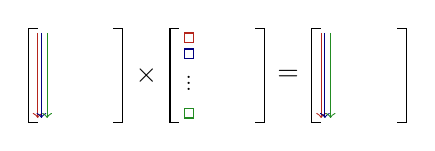
\begin{tikzpicture}[scale=1.2]
        \draw (-1.25,-0.5) -- (-1.25,0.5);
        \draw (-1.25,-0.5) -- (-1.15,-0.5);
        \draw (-1.25,0.5) -- (-1.15,0.5);
        \draw (-0.25,-0.5) -- (-0.25,0.5);
        \draw (-0.25,-0.5) -- (-0.35,-0.5);
        \draw (-0.25,0.5) -- (-0.35,0.5);

        \node at (0,0) () {$\times$}; 

        \draw (1.25,-0.5) -- (1.25,0.5);
        \draw (1.25,-0.5) -- (1.15,-0.5);
        \draw (1.25,0.5) -- (1.15,0.5);
        \draw (0.25,-0.5) -- (0.25,0.5);
        \draw (0.25,-0.5) -- (0.35,-0.5);
        \draw (0.25,0.5) -- (0.35,0.5);

        \node at (1.5,0) () {$=$};

        \draw (2.75,-0.5) -- (2.75,0.5);
        \draw (2.75,-0.5) -- (2.65,-0.5);
        \draw (2.75,0.5) -- (2.65,0.5);
        \draw (1.75,-0.5) -- (1.75,0.5);
        \draw (1.75,-0.5) -- (1.85,-0.5);
        \draw (1.75,0.5) -- (1.85,0.5);

        \draw[color=BrickRed, ->] (-1.15,0.45) -- (-1.15,-0.45);
        \draw[color=NavyBlue, ->] (-1.11,0.45) -- (-1.11,-0.45);
        \draw[color=ForestGreen, ->] (-1.05,0.45) -- (-1.05,-0.45);

        \draw[color=BrickRed] (0.4,0.35) rectangle (0.5,0.45);
        \draw[color=NavyBlue] (0.4,0.18) rectangle (0.5,0.28);
        \node[rotate=90] at (0.45,-0.085) () {\scriptsize{...}};
        \draw[color=ForestGreen] (0.4,-0.45) rectangle (0.5,-0.35);

        \draw[color=BrickRed, ->] (1.85,0.45) -- (1.85,-0.45);
        \draw[color=NavyBlue, ->] (1.89,0.45) -- (1.89,-0.45);
        \draw[color=ForestGreen, ->] (1.95,0.45) -- (1.95,-0.45);
    \end{tikzpicture}
\end{figure}